\section{Problématique de la reconstruction de signal}
La reconstruction du signal est un problème que l'on considère dans le cadre du traitement du signal, c'est à dire que l'on considère qu'à un signal, on peut appliquer une transformation, et de cette transformation on obtient un nouveau signal qui aura certaines caractéristiques permettant de mieux comprendre ce signal.
D'un point de vue plus formel, on considère une famille de signaux $\mathcal{F}$, chaque élément de cette famille étant une application $f : X \longrightarrow Y$, et on considère un opérateur $A : \mathcal{F} \longrightarrow \mathcal{G}$, où $\mathcal{G}$ est une autre famille de signaux.
Donnons ici quelques exemples de familles de fonctions que l'on rencontrera dans ce mémoire. Commencons avec les fonctions à temps continu (c'est à dire avec $X = \mathbb{R}^d$ pour un certain $d>0$).
%%TODO : remplacer d par N pour être cohérent avec la suite
\begin{exemple}
	Signaux à énergie finie :
	\begin{enumerate}
		\item $\mathcal{F} = L^2(\mathbb{R}^d) := \{f : \mathbb{R}^d \longrightarrow \mathbb{R} | \int_\mathbb{R}^d |f(t)|^2dt < \infty\}$.
		\item $\mathcal{F} = L^p(\mathbb{R}^d) := \{f : \mathbb{R}^d \longrightarrow \mathbb{R} | \int_\mathbb{R}^d |f(t)|^pdt < \infty\}$, pour $0 < p \leq 1$.
		\item $\mathcal{F} = L^\infty(\mathbb{R}^d) := \{f : \mathbb{R}^d \longrightarrow \mathbb{R} | \sup_{t\in \mathbb{R}^d} |f(t)| < \infty\}$.
	\end{enumerate}
	Signaux avec une régularité :
	\begin{enumerate}
		\item $\mathcal{F} = \mathcal{C}^0(\mathbb{R}^d) =\{f : \mathbb{R}^d \longrightarrow \mathbb{R} \text{avec } f \text{ continue}\}$.
		\item $\mathcal{F} = \mathcal{C}^r(\mathbb{R}^d) =\{f : \mathbb{R}^d \longrightarrow \mathbb{R} \text{avec } \forall t \in \mathbb{R}^d \sup_{0\leq k \leq r} | f^{(k)}(t)| < \infty$.
	\end{enumerate}
\end{exemple}
on pourra aussi considérer pour chacun des espaces ci-dessus, leur version à support compact, notée avec l'indice $_\text{loc}$ (par exemple $L^p_\text{loc}$ ou $\mathcal{C}^p_\text{loc}$ ) pour indiquer que pour tout $f\in \mathcal{F}_\text{loc}$, il existe un $C \geq 0$ tel que $\lvert t \rvert \geq C \implies f(t) = 0$. On considérera également des càs où $X$ est un ouvert ou un fermé de $\mathbb{R}^d$
Un autre espace qui sera peut être utilisé est l'espace de Sobolev $W^{r, p}$ qui représente des signaux à énergie finie pour $||\cdot|| _p$, mais dont chaque dérivéé (définie faiblement) d'ordre inférieur ou égal à $r$ est elle aussi à énergie finie.
\newline
Une autre classe d'intérêt de signaux majeur est celle des signaux à temps discret (c'est à dire avec $X = \mathbb{N}^d$).
\begin{exemple}
	Signaux à énergie finie :
	\begin{enumerate}
		\item $\mathcal{F} = l^2(\mathbb{N}^d) := \{f : \mathbb{N}^d \longrightarrow \mathbb{R} | \sum_\mathbb{N}^d |f(t)|^2 < \infty\}$.
		\item $\mathcal{F} = l^p(\mathbb{N}^d) := \{f : \mathbb{N}^d \longrightarrow \mathbb{R} | \sum_\mathbb{N}^d |f(t)|^p < \infty\}$, pour $0 < p \leq 1$.
		\item $\mathcal{F} = l^\infty(\mathbb{N}^d) := \{f : \mathbb{N}^d \longrightarrow \mathbb{R} | \sup_{t\in \mathbb{N}^d} |f(t)| < \infty\}$.
	\end{enumerate}
\end{exemple}
On verra plus loin que l'on peut également définir une notion de régularité intéressante pour les signaux à temps discret.
\begin{remarque}
	Dans les exemples ci-dessus les signaux sont à valeur dans $Y = \mathbb{R}$, cependant toutes ces exemples peuvent être considérées avec $\mathbb{C}$ comme espace d'arrivée. 
\end{remarque}

\subsection{Exemples de signaux étudiés (image, sons, tomographie, ...) et formalisation mathématique de leur description}
Considérons maintenant de façon plus concrète des exemples de signaux étudiés afin d'introduire l'opérateur $A$.
\newline
TODO : Pour chacun des exemples ci-dessous, formaliser le problème et poser sa solution comme un problème de minimisation "$argmin$"

\begin{exemple} L'exemple le plus simple pour introduire le sujet est celui d'un signal à une dimension, on pourra par exemple penser à un signal décrivant un son ou bien un signal electrique, d'une durée finie, et à chaque instant on peut associer une amplitude. D'un point de vue formel on pourra ainsi considérer que ce signal est $f:[0, 1] \longrightarrow \mathbb{R}^+$. On pourra cherche à faire différentes opérations sur ce signal :
	\begin{itemize}
		\item \it{Echantillonage}
		\item \it{Seuil}
		\item \it{Décomposition harmonique (Fourier)}
		\item \it{Filtrage}
	\end{itemize}
\end{exemple}
\begin{exemple}
	Après avoir considéré le signal à une dimension, un autre type de signal est celui des signaux en deux ou trois dimensions  dimensions dont l'exemple type est celui des vidéos ou des images :
	\begin{itemize}
		\item \it{Débruitage}
		\item \it{Super-résolution}
		\item \it{Compression}
		\item \it{Détection / Reconnaissance}
	\end{itemize}
\end{exemple}
\begin{exemple}
	Une autre problématique essentielle que l'on considérera en profondeur dans ce mémoire est celui des problèmes inverses dans lesquels à partir d'un signal mesuré, on cherchera à reconstruire ce qui a émis ce signal.
	\begin{itemize}
		\item \it{Tomographie (transformée de Radon)} 
		\item \it{Géologie/IRM}
	\end{itemize}  
\end{exemple}
\begin{exemple}
	Récemment, des problèmes avec des signaux en grande dimension sont aussi apparus, notamment dans des problématiques de type big-data.
\end{exemple}

Cependant sur ces problèmes il y a une ambiguité sur la définition de la dimension qui est considérée comme la dimension de l'espace de départ du signal considéré, mais cependant, chaque signal appartient à un espace qui n'a à priori aucune raison d'être fini. 
De plus, chacun de ces problèmes commence par une mesure qui est toujours un processus discret et le reste du traitement est réalisé sur un ordinateur qui est lui aussi un processus discret.
Ainsi chacun de ces problèmes est discretisé et alors la dimension\footnote{On considère ici la "dimension" comme étant le nombre de degré de libertés du signal étudié.} du signal augmente de façon considérable, ainsi, une image photographie a typiquement une dimension $d >> 10^6$.

\section{Exactitude, échantillonage et bruit}
\subsection{Lien entre l'exactitude et l'échantillonage}
Ainsi il est nécessaire d'adapter la stratégie d'échantillonage, un échantillonage insuffisant ou inaproprié ne permettra pas avec certitude de pouvoir récupérer l'information sous-jacente au signal.
Un échantillonage qui prendrait trop de mesures pose aussi des problèmes, premièrement car si la taille de ces mesures est trop importante, il sera difficile de faire des opérations dessus et cela compliquera la résolution du problème. 
Mais aussi, car augmenter le nombre de mesures risque de ne pas apporter davantage d'informations pour la résolution du problème \footnote{On peut ici penser aux problématiques d'\it{overfitting} du Machine Learning dans lesquels un système qui est trop entrainé sur un ensemble de données devient inefficace dès qu'il est testé sur des données sur lesquelles il n'a pas été entrainé}
, et dans certains cas, ces mesures superflues risquent seulement de mesurer du bruit et donc de diminuer l'efficacité de la résolution.
Il est donc nécessaire pour une famille de signaux donnée d'avoir des conditions nécessaires sur l'échantillonage, pour veiller à être certain d'étudier au moins le signal, mais aussi des conditions suffisantes pour ne pas étudier trop au delà du signal.
\subsection{L'importance du bruit dans les problèmes}
Ainsi il est nécessaire de prendre en compte le fait qu'il y ait des sources de bruit dans les problèmes considérés et on cherchera donc à vérifier que les constructions qui viendront seront stables face au bruit.
Une remarque importante à faire est que le bruit est généralement constitué de modifications très locales (que l'on considérera ainsi comme "hautes-fréquences").

\section{Bases orthonormales et frames}
\subsection{Intérêt des bases orthonormales et description des outils mathématiques disponibles}
Une approche classique et pratique pour l'analyse de signaux est l'utilisation d'une base orthonormale pour représenter un signal. 
En effet l'intérêt est multiple, si l'on connait une base orthonormale de décomposition d'un signal, alors il y aura une unique façon d'écrire ce signal dans cette base, mais surtout, l'espace est alors naturellement muni d'un produit scalaire qui permettra d'utiliser tout l'outillage des espaces de Hilbert pour résoudre le problème.
\newline
On verra ainsi dans cette section tout d'abord des définitions et propriétés classiques des espaces de Hilbert. 
Ensuite on verra progressivement comment relacher certaines des définitions initiales afin de pouvoir conserver une formule de reconstruction.
Afin d'expliciter l'intérêt de ces définitions on verra deux exemples de frames.
Tout d'abord le frame de Fourier, dont la compréhension sera utile pour le troisième chapitre.
Finalement, nous introduirons les ondelettes par l'analyse multi-résolution, les formules que nous obtiendrons seront utilisées dans le chapitre suivant.
\subsection{Lien entre frames et base orthonormale}
Rappelons tout d'abord les définitions et propriétés d'une base orthonormale. On considère ici un espace $H$ muni d'un produit scalaire et une famille $\{e_i\}_I$, avec $I$ un ensemble.
\begin{definition}
	On dira qu'une famille $\{e_i\}_I$ est :
	\begin{itemize}
		\item \it{libre} si pour n'importe quelle suite finie de coefficients $(\lambda_i)_I$ telle que $\sum_I \lambda_i e_i = 0$, on a $\lambda_i = 0$ pour n'importe quel $i \in I$.
		\item \it{orthogonale}\footnote{Dans un espace vectoriel muni d'un produit scalaire et d'une base, une famille est libre si et seulement si elle est orthogonale (cela découle des propriétés du produit scalaire, notamment qu'il est défini).} si pour n'importe quels $i$ et $j$ différents on a $\langle e_i, e_j \rangle = 0$
		\item \it{génératrice} si quel que soit $f \in H$ tel que pour tout $i\in I$ on a $\langle f, e_i \rangle = 0$, alors $f =0$.
		\item une \it{base} si la famille est libre et génératrice.
	\end{itemize}
\end{definition}
Donc, pour tout $h \in H$, si la famille $\{e_i\}_I$ est libre et génératrice, il existe une unique suite $(\lambda_i)_{i \in I}$ de scalaires, telle que $ h = \sum_{i \in I} \lambda_i e_i$.
On peut alors définir un nouveau produit scalaire sur $H$: 
\begin{align}
	\langle \cdot, \cdot \rangle :  H \times H &\longrightarrow \mathbb{R} \\
		(h_1= (\lambda_i)_I, h_2 = (\mu_i)_I) &\longmapsto \langle h_1, h_2 \rangle = \sum_I \lambda_i \mu_i^*.
\end{align}
On peut remarquer que ce produit scalaire est défini de façon unique par rapport à la base $\{e_i\}_I$, cependant, si la base est normalisée ($\langle e_i, e_i \rangle =1$), alors ce produit scalaire devient identique au produit scalaire initial de $H$. 
Ainsi, la valuation du produit scalaire est indépendante du choix de la base (tant qu'elle est normalisée)\footnote{Dans $L^2(\mathbb{R})$, on peut ainsi retrouver les égalités de Parseval ou de Plancherel en exprimant une fonction $f\in L^2(\mathbb{R})$ soit dans la base canonique de $L^2(\mathbb{R})$ par rapport à $f$ donnée par le vecteur $\frac{f}{||f||}$et une base de son orthogonal, soit en exprimant la fonction dans la base de Fourier.}.
On a alors le théorème suivant qui nous donne une condition nécessaire et suffisante pour que l'espace engendré par une famille $\{f_i\}$ soit dense dans H:
\begin{theoreme}
	Soit $\{f_i\}_I$ une suite d'éléments orthonormaux dans $H$ muni d'un produit scalaire.
	Alors $\overline{\text{Vect}(\{f_i\}_I)} = H$ si et seulement si 
	\begin{equation*}
		\sum_I |\langle f, f_i\rangle|^2 = ||f||_2 ^2 \quad, \forall f \in H.
	\end{equation*}
\end{theoreme}
Cependant, comme on le verra dans la suite, il y a des situations dans lesquelles chercher à avoir une base orthonormale est trop restrictif, on cherchera donc à relacher les conditions sur la définition d'une base.
\newline
Tout d'abord, si la famille est orthogonale, mais elle n'est pas génératrice on a 
\begin{theoreme}
	Soit $\{f_i\}_I$ une famille orthonormale de $H$.
	Alors,
	\begin{equation*}
		\sum_I |\langle f, f_i \rangle|^2 \leq ||f||_2 ^2, \forall f \in H
	\end{equation*}.
\end{theoreme}
On peut exprimer ce théorème en disant que l'analyse par une famille orthogonale n'ajoute pas d'énergie au vecteur analysé.
et si la famille est génératrice,
\begin{theoreme}
	Soit $\{f_i\}_I$ une famille génératrice normalisée.
	Alors,
	\begin{equation*}
		||f||^2 \leq \sum_I |\langle f, f_i \rangle|^2, \forall f \in H
	\end{equation*}.
\end{theoreme}
On peut exprimer ce théorème en disant que l'analyse par une famille génératrice capture au moins l'énergie du vecteur analysé.
Au vu de ces résultats, on est amenés à considérer les définitions suivantes qui correspondent à une relaxation de la condition de normalisation ou de la condition d'orthogonalité.
\begin{definition}
	Pour une famille d'éléments $\{f_i\}_I$ de $H$, alors on dit que c'est 
	\begin{enumerate}
		\item Une suite de \it{Bessel} si il existe une constante $M>0$ telle que
			\begin{equation*}
				\sum_I |\langle f, f_i \rangle|^2 \leq M||f||^2, \forall f \in H.
			\end{equation*}
		\item Un \it{frame} si il existe des constantes $M, m>0$ telles que
			\begin{equation}\label{eq:defFrame}
				m||f||^2 \leq \sum_I |\langle f, f_i\rangle|^2 \leq M||f||^2, \forall f \in H.
			\end{equation}
		\item Une \it{base de Riesz} (ou base \it{inconditionnelle}) si il existe des constantes $M, m>0$ telles que
			\begin{equation*}
				m\sum |c_k|^2 \leq ||\sum c_k f_k||^2 \leq M\sum |c_k|^2
			\end{equation*}
		pour n'importe quelle suite finie $\{c_k\}$.
	\end{enumerate}
\end{definition}
\begin{remarque}
	\begin{itemize}
		\item Une base orthonormale est une base de Riesz avec $m = M = 1$.
		\item Une base de Riesz est un frame dont les éléments sont linéairement indépendents.
		\item Un frame est une suite de Bessel dont les éléments sont générateurs.
	\end{itemize}
\end{remarque}
Ainsi, lorsque l'on dispose d'une suite $F = \{f_i\}_I$ on peut définir l'opérateur d'analyse
\begin{equation*}
	\theta_F (f) = \{\langle f, f_i \rangle\}_I 
\end{equation*}
et de synthèse
\begin{equation*}
	\theta^*_F( \{c_i\}_I) = \sum_I c_i f_i.  
\end{equation*}
Ainsi la composée des deux opérateurs nous donne un opérateur de projection dans l'espace vectoriel engendré par $F$ :
\begin{equation}\label{eq:thetaF}
	\theta^*_F \circ \theta_F (f) = \sum_I \langle f, f_i\rangle f_i. 
\end{equation}
Tout d'abord on peut remarquer que, si $F$ est une famille orthogonale, alors l'application précédente correspond presque à une projection orthogonale dans l'espace engendré par $F$\footnote{La propriété qui n'est pas vérifiée est $(\theta^*_F \circ \theta_F)^2 = Id_{Vect(F)}$}.
On va maintenant voir que si $F$ est un frame \textit{équilibré} (c'est à dire avec des constantes $m, M$ égales), alors on dispose d'une formule analogue à \ref{eq:thetaF} qui nous donne une projection orthogonale.
L'intérêt de cela étant que, si $F$ est génératrice de l'espace entier $H$, alors la projection orthogonale correspond à une formule de reconstruction.
\newline
Supposons ainsi que l'on ait $m =M$, on a d'après \ref{eq:defFrame}, 
\begin{equation*}
	\sum_I |\langle f_j, f_i \rangle |^2 = M||f_j||^2.
\end{equation*}
Posons $\pi = \frac{1}{M}\theta^*_F \circ \theta$ et vérifions que c'est une projection orthogonale, soit $f\in Vect(F)$, alors
$f = \sum_J \lambda_j f_j$ avec $J\subset I$, d'où,
\begin{equation*}
	\langle f, f_k \rangle = \sum_J \lambda_j \langle f_j, f_k \rangle = \lambda_k \langle f_k, f_k \rangle + \sum_{j \in J-\{k\}} \lambda_j \langle f_j, f_k \rangle  
\end{equation*}
\begin{equation*}
	\pi(f) = \frac{1}{M}\sum_I \langle f, f_i \rangle f_i 
	= \frac{1}{M}\sum_J \lambda_j \sum_I \langle f_j, f_i \rangle f_i  
\end{equation*}
et pour conclure, on projète $\pi(f)$, sur chaque composante $f_k$ et on obtient
\begin{align*}
	\langle \pi(f), f_k \rangle &= \frac{1}{M} \sum_J \lambda_j \sum_I \langle f_j, f_i \rangle \langle f_i, f_k \rangle 
	= \frac{1}{M}  \lambda_k \sum_I |\langle f_k, f_i\rangle|^2 + \frac{1}{M} \sum_{j \in J-\{k\}}\lambda_j \sum_I  \langle f_j, f_i \rangle \langle f_i, f_k \rangle \\
	&= \frac{1}{M} \lambda_k M \langle f_k, f_k \rangle + \frac{1}{M} \sum_{j \in J-\{k\}} \lambda_j M\langle f_j, f_k \rangle \\
	&= \langle f, f_k \rangle.
\end{align*}
On a donc, si $f$ est dans l'espace engendré par F, alors la projection ne change pas les coordonées de $f$, sinon, si $f$ est dans l'orthogonal de $F$, alors chacune de ses composantes est orthogonale à tous les $f_i$, donc $f$ est dans le noyau de $\pi$.
Ainsi, $\pi$ est bien une projection orthogonale dans $F$.
\newline
On dispose donc d'une formule de reconstruction qui est valable pour tout $f$ qui est dans l'espace engendré par $F$ 
\begin{equation}
	f = \frac{1}{M} \sum_{f_i \in F} \langle f, f_i \rangle f_i 
\end{equation}
cependant cette formule ne semble rajouter que des complications par rapport à une base orthonormale (cas $m=M=1$ d'après la combinaison des théorèmes \ref{th:orth1} et \ref{th:norm1}). 
Nous allons donc voir ci-dessous en quoi avoir un coefficient de frame équilibré $M>1$ permet d'améliorer la stabilité de la formule de reconstruction, on appelera un tel frame redondant.
Ainsi, comme aperçu par Jean Morlet dès 1986 (TODO: ajouter ref Daubechies) travailler avec des frames permet, en pratique, de pouvoir stocker des coefficients de frame avec moins de précision.
Avant de poursuivre et de prouver cette observation de Jean Morlet, voyons d'abord rapidement comment obtenir la redondance d'un frame équilibré d'un point de vue formel.
Soit $F=(f_i)_{i=1, \cdots, N}$ un frame équilibré et on considère $Vect(F)$ l'espace vectoriel engendré par $F$, qui est un espace vectoriel de dimension $d$. 
Si les éléments de $F$ ne sont pas linéairement indépendants, alors on a $d<N$ et $M>1$.
Montrons avec le lemme suivant la relation entre le nombre d'éléments dans un frame équilibré ($N$), la constante de frame ($M$) et la dimension de l'espace engendré par le frame ($d$).
\begin{lemme}
	Soit $\Phi =(\varphi_i)_{i=1, \cdots, N}$ un frame avec des constantes de frame $m=M$ qui engendre $Vect \Phi$ un espace vectoriel de dimension $d$.
	Alors
	\begin{equation}
		\frac{N}{M^2} \leq d?
	\end{equation}
\end{lemme}
\begin{proof}
	Afin de prouver ce résultat rappelons que l'on a l'opérateur d'analyse
	\begin{align}
		\mathbb{R}^d &\longrightarrow^A \ell^2(N)\\
		f \longmapsto (\langle f, \varphi_i \rangle)_{i=1,\cdots, N}
	\end{align}
	et le frame étant équilibré, la boule $B_d(0,1)$ dans $\mathbb{R}^d$ de rayon 1 est envoyée sur la boule $B_N(0,M)$ de $\ell^2(N) := \ell^2(\{0, \cdots, N\})$.
	Maintenant, on considère l'opérateur de synthèse,
	\begin{align}
		\ell^2(N) &\longrightarrow^S \mathbb{R}^d\\
		x=(x_i)_{i=1, \cdots, N} &\longmapsto \sum_{i=1}^N x_i \varphi_i
	\end{align}
	et on considère, sans perte de généralité que chaque $\varphi_i$ est normalisé. Ainsi chaque à chaque $\varphi_i$, on peut associer une suite $(\lambda_j^i)_{j=0, \cdots, d}=(\langle \varphi_i, e_j)_{j=0,\cdots, d}$ de norme 1 dans $\mathbb{R}^d$ muni de la norme euclidienne telle que $\varphi_i = \sum_{j=1}^d \lambda_j^i e_j$ où $e_j$ est une base orthonormale de $\mathbb{R}^d$. 
	L'objectif est maintenant de réécrire $S(x)$ dans la base orthonormale, on a ainsi
	\begin{equation}
		\sum_{i=1}^N x_i \varphi_i = \sum_{i=1}^N x_i \sum_{j=1}^d \lambda_j^i e_j = \sum_{j=1}^d \sum_{i=1}^N x_i \lambda_j^ie_j =\sum_{j=1}^d c_j e_j,
	\end{equation}
	où $c_j = \sum_{i=1}^Nx_i\lambda_j^i$. On va maintenant majorer les $c_j$ de façon uniforme, chaque $\lambda_j^i$ correspond à la projection de $\varphi_i$ sur $e_j$, chaque $\varphi_i$ est dans la boule unité ainsi $c_j$ correspond à la projection de tous les $\varphi_i$ sur $e_j$, ainsi on a la majoration
	\begin{equation}
		c_j \leq ||x||_2 M.
	\end{equation}
	On a maintenant la majoration,
	\begin{equation}
		||S (x)||^2_2 = ||\sum_{j=1}^d c_j e_j||_2^2= \sum_{j=1}^d c_j^2 \leq d M^2||x||_2^2. 
	\end{equation}
	On va maintenant chercher une minoration de $||S(x)||_2^2$,
	\begin{equation}
		||S(x)||_2^2 = ||\sum_{i=1}^N x_i \sum_{j=1}^d \lambda_j^i e_j||_2^2 \geq N||x||_2^2 \min_{i=1, \cdots, N} ||\sum_{j=1}^d \lambda_j^i e_j||_2^2 = N||x||_2^2 \min_{i=1, \cdots, N}\sum_{j=1}^d (\lambda_j^i)^2.
	\end{equation}
	Or,
	\begin{equation}
		\sum_{i=1}^d (\lambda_j^i)^2 = \sum_{i=1}^d |\langle \varphi_j, e_i \rangle|^2 =||\varphi_j||_2^2=1.  
	\end{equation}
	On peut donc combiner les inégalités obtenues et on a
	\begin{equation}
		N ||x||_2^2 \leq ||S(x)||_2^2 \leq d M^2||x||_2^2
	\end{equation}
	et ainsi
	\begin{equation}
		\frac{N}{M^2} \leq d.
	\end{equation}
\end{proof}
Fixons maintenant un élément $f\in  Vect(F)$,
supposons tout d'abord que l'on est dans le cas classique où ${e_i}_{i=1, \cdots, d}$ est une base orthonormale de $Vect(F)$, on a ainsi la formule standard,
\begin{equation*}
	f = \sum_{i=1}^d \langle f, e_i \rangle e_i = \sum_{i=1}^d c_i e_i
\end{equation*}
Maintenant perturbons les coefficients de la façon suivante, fixons un $\epsilon >0$ qui nous permettra de contrôler la taille de la perturbation introduite, et prenons $d$ variables aléatoires réelles indépendantes $(\alpha_i)_{i=1,\cdots, d}$ de moyenne nulle et de variance égale à 1.
On peut alors perturber chaque coefficient $c_i$ en y ajoutant $\epsilon \alpha_i$, on peut alors calculer l'erreur de reconstruction moyenne
\begin{align*}
	\mathbb{E}\left(|| f- \sum_{i=1}^d (c_i + \epsilon \alpha_i)e_i||_2^2\right) &= \mathbb{E}\left(\sum_{i=1}^d \epsilon^2 \alpha_i^2\right)\\
		&= \epsilon^2 \sum_{i=1}^d \mathbb{E} (\alpha_i^2) = \epsilon^2 d.
\end{align*} 
Maintenant appliquons la même altération aux coefficients de $f$ dans le frame $F$ afin de calculer l'erreur de reconstruction moyenne.
Ainsi, on a la formule de reconstruction
\begin{equation*}
	f = \frac{1}{M}\sum_{i=1}^N \langle f, f_i \rangle f_i
\end{equation*}
et prenons $N$ variables aléatoires réelles indépendantes $(\alpha_i)_{i=1, \cdots, N}$  de moyenne nulle et de variance égale à 1.
\begin{align*}
	\mathbb{E}\left(|| f- \frac{1}{M}\sum_{i=1}^N (\langle f, f_i\rangle + \epsilon \alpha_i)e_i||_2^2\right) &= \mathbb{E}\left(||\frac{1}{M} \sum_{i=1}^N \epsilon \alpha_i||_2^2\right)\\
	&= \frac{\epsilon^2}{M^2} \mathbb{E}(\sum_{i=1}^N \alpha_i^2) = \frac{\epsilon^2 N}{M^2}.	
\end{align*}
Ainsi, d'après le lemme précédent, l'erreur de reconstruction moyenne d'un frame redondant est toujours au moins aussi petite que l'erreur de reconstruction dans une base orthonormale.
Montrons avec un exemple dans $\mathbb{R}^2$ que l'on peut faire mieux que le résultat du lemme.
Soit $\varphi_1 = (0, 1), \varphi_2 = (-\frac{\sqrt{3}}{2}, -\frac{1}{2}), \varphi_3 =(\sqrt{3}{2}, -\frac{1}{2})$ et prenons $x=(x_1, x_2)$ un élément de $\mathbb{R}^2$, alors,
\begin{align*}
	\sum_{i=1}^3 |\langle x, \varphi_i \rangle|^2 &= |x_2|^2 + |-\frac{\sqrt{3}}{2}x_1 -\frac{1}{2} x_2|^2 + |\frac{\sqrt{3}}{2}x_2 - \frac{1}{2}x_1|2 \\
	&= \frac{3}{2}(|x_1|^2 + |x_2|^2) = \frac{3}{2} ||x||_2^2.
\end{align*}
Ainsi, les vecteurs $(\varphi_1, \varphi_2, \varphi_3)$ forment un frame équilibré de constante $M=\frac{3}{2}$ de $\mathbb{R}^2$.
On a alors $\frac{N}{M^2} = \frac{3}{M^2} = \frac{4}{3} < 2 = d$.
Donc dans le cas de ce frame, l'erreur de reconstruction moyenne après perturbation des coefficients est améliorée d'un facteur $\frac{2}{3}$ par rapport à celle que l'on obtiendrait en utilisant une base orthonormale de $\mathbb{R}^2$.

\subsection{Exemples de frames (Fourier, ondelettes)}
Introduisons maintenant la décomposition d'une fonction en ondelettes.
\begin{definition}
	On dit que $\psi:\mathbb{R} \to \mathbb{R}$ est une ondelette génératrice si 
	\begin{equation}
		\{\psi_{j,k} := 2^{j/2}\psi(2^j\cdot - k)\}_{j,k \in \mathbb{Z}}
	\end{equation}
	est une famille génératrice de $L^2(\mathbb{R})$.
	On appelera\footnote{On considérera par la suite des frames d'ondelettes ou bien des bases de Riesz d'ondelettes} une base engendrée par une telle fonction $\psi$ une base d'ondelettes.
\end{definition}
\begin{figure}
	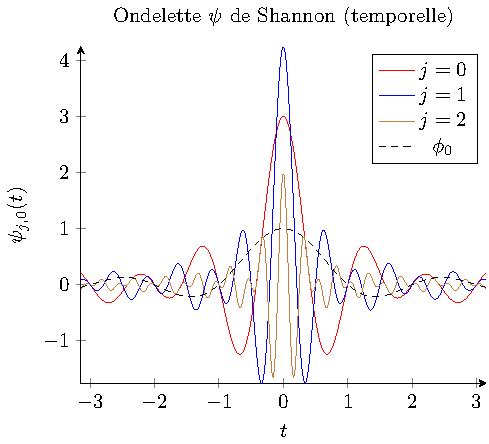
\includegraphics{Figs/shannon}
\end{figure}
\begin{remarque}
	Dans la définition des ondelettes $\psi_{j,k}$ engendrées par $\psi$, le coefficient $j$ correspond au facteur d'échelle\footnote{Du point de vue des notations, on considère que $j$ tend vers l'infini, signifie que $\psi_j$ analyse les hautes fréquences, ce choix de notation n'est pas uniforme dans la littérature, par exemple (TODO :ajouter ref) Mallat et Daubechies, utilisent $-j$ par rapport à nos notations. Par contre les notations utilisées correspondent à celles de Jaffard et Meyer. Mais cependant tous les résultats sont bien entendu équivalents.},
	en raison du facteur $2^j$ devant la variable, au fur et à mesure que $j$ augmente, l'ondelette est parcourue de plus en plus vite. Ainsi, augmenter $j$ revient à augmenter la fréquence de $\psi$, c'est à dire d'éloigner le support de $\hat{\psi}$ de l'origine\footnote{En effet, de façon plus précise et formelle, on a $\hat{\psi_{j,0}}(\omega) = 2^{-\frac{j}{2}}\hat{\psi}(\frac{\omega}{2^j})$.}.
	Le coefficient $k$ correspond à une translation de l'ondelette $\psi_j$, en ce sens, l'analyse par ondelette, permet une analyse à la fois en temps (par rapport à $k$) et en fréquence (par rapport à $j$).
\end{remarque}
Donc étant donnée une famille d'ondelettes $\{\psi_{j,k}\}_{j,k \in \mathbb{Z}}$, on peut associer à une fonction $f\in L^2(\mathbb{R})$, ses coefficients d'ondelettes
\begin{equation}
	Wf = (\langle f, \psi_{j,k} \rangle )_{j,k \in \mathbb{Z}}
\end{equation}
et on se demande alors si à partir de ces coefficients on peut reconstruire $f$.
Cela revient ainsi à déterminer si la famille d'ondelettes est un frame d'ondelette. 
Ici on ne cherchera pas a énumérer et a vérifier des frames d'ondelettes, un très grand nombre de frames d'ondelettes existent (ajouter ref.), on admet ainsi pour l'instant l'existence des frames d'ondelettes.
Un peu plus bas nous verrons et démontrerons un théorème qui permet de construire de nombreux frames d'ondelettes, ce théorème fournira également une extension des ondelettes à $L^2(\mathbb{R}^d)$ et avec une version qui montre que la présence de puissances de 2 dans la définition des ondelettes revient à un choix d'échantillonage. 
\newline
Supposons ainsi que l'on dispose d'un frame d'ondelettes et que ce frame est équilibré (c'est à dire que les bornes de frame $m$ et $M$ sont égales), alors on dispose d'une formule de reconstruction (d'après Daubechies 3.2.2)
\begin{equation}
	f = \frac{1}{M} \sum_{j,k} \langle f, \psi_{j,k}\rangle \psi_{j,k}.
\end{equation}
Cependant bien que la formule précédente permette une reconstruction elle suppose de parcourir des indices sur $\mathbb{Z}$ ce qui pourrait créer des complications concernant la convergence (d'un point de vue théorique ou pratique).
On va ici très rapidement introduire la notion d'analyse multi-échelle qui permet de simplifier la formule de reconstruction.
Construisons ici une analyse multi-échelle (ici de $L^2(\mathbb{R})$), considérons tout d'abord une suite d'espaces emboités satisfaisant 
\begin{equation*}
	\{0\}=	\lim_{j\to -\infty} \bigcap_{j}^{+\infty} V_i \subset \cdots \subset V_{-1} \subset V_0 \subset \cdots V_i \subset V_{i+1} \subset \cdots \subset \lim_{j\to \infty} \bigcup_{-\infty}^{j} V_i = L^2(\mathbb{R}).  
\end{equation*}
L'intérêt d'avoir une telle suite d'espaces emmboités est que étant donnée une fonction $f\in L^2(\mathbb{R})$, on peut considérer sa projection orthogonale dans un $V_i$, on a alors une approximation $f_i$ de $f$ dans $V_i$, si on souhaite améliorer l'approximation de $f$ il suffit alors de remonter dans ces espaces emboités pour avoir une reconstruction avec une précision arbitraire.
Introduisons maintenant la propriété qui va permettre de voir cette suite d'espaces comme une analyse multi-échelle
\begin{equation}
	f(\cdot) \in V_j \iff f(\frac{\cdot}{2^j}) \in V_0,
\end{equation}
c'est à dire que les fonctions d'un espace $V_j$ sont des versions dilatées d'un facteur $2^{-j}$ des fonctions de l'espace $W_0$.
Ajoutons maintenant la condition que $V_0$ contient toutes les translations entières de ses éléments, c'est à dire
\begin{equation}
	f \in V_0 \iff f(\cdot - n) \in V_0 \forall n \in \mathbb{Z}.
\end{equation}
Ainsi, une fonction qui appartient à $V_j$ s'écrit comme une combinaison linéaire de versions translatées et dilatées de fonctions appartenant à $V_0$.
De plus, quelque soit $j$ on peut prendre $W_j$ le complémentaire orthogonal de $V_j$ dans $V_{j+1}$, 
\begin{equation}
	f = \pi_{V_0}(f) +\sum_{i>0} \pi_{W_j}(f) 
\end{equation}
donc afin d'avoir une formule de reconstruction, il suffit de connaitre un frame de $V_0$ et de même pour chaque $W_j$. 
On peut maintenant revenir aux ondelettes, on considère que l'on connait une base $(\varphi_{0,k})_{k\in \mathbb{Z}}$ de $V_0$ et $(\psi_{j,k})_{j\in \mathbb{N}^*, k \in \mathbb{Z}}$ un frame de l'orthogonal de $V_0$ dans $L^2(\mathbb{R})$, on pose alors $W_j = W_{j-1} \bigoplus Vect(\{\psi_{j,k}\}_{k\in \mathbb{Z}})$ et on obtient ainsi que l'analyse multi-échelle ainsi construite fournit une formule de reconstruction\footnote{Dans la formule de reconstruction les deux sommes sur $\mathbb{Z}$ ne sont pas problématiques car les fonctions considérées sont dans $L^2(\mathbb{R})$ donc avec une décroissance suffisament rapide, donc seulement un nombre fini de $\langle f, \varphi_{0,k} \rangle$ sont différents de 0 si $\varphi_0$ a une décroissance suffisament rapide (et de même pour chaque $\psi_j$).}
\begin{equation}
	f = \sum_{k\in \mathbb{Z}} \langle f, \varphi_{0,k} \rangle \varphi_{0,k} + \sum_{j = 1}^{+\infty} \sum_{k\in \mathbb{Z}} \langle f, \psi_{j,k} \rangle \psi_{j,k}.
\end{equation}
On appelle l'application $\varphi_0$ ondelette d'échelle.
On a vu que les familles orthonormales forment des frames, on a donc la proposition :
\begin{proposition}
	\begin{enumerate}
		\item La transformée de Fourier discrète est un frame pour $\mathcal{F}$.
		\item Les ondelettes forment un frame pour $\mathcal{F}$.
	\end{enumerate}
\end{proposition}
\begin{preuve}
	\begin{enumerate}
		\item On utilisera la transformée de Fourier discrète écrite sous forme de matrice unitaire, qui est une matrice unitaire de Vandermonde avec les racines de l'unité en coefficients. Avec de l'algèbre on montre l'orthonormalité des colonnes.
		\item Application du théorème suivant.
	\end{enumerate}
\end{preuve}

\begin{theoreme}
	Soit $\mathcal{Q} \subset \mathcal{R}^d$ un ensemble de mesure finie, $h \in L^2(\mathbb{R}^d)$
	et $\mathcal{A} =\{A_j \in GL_d(R)\}_J$ une famille de matrices inversibles.
	\newline
	Pour tout $j \in J$, on pose $B_j =(A_j^T)^{-1}, S_j = A_j^TQ, h_j = h(B_j \cdot)$
	et soit $\mathcal{S} = \{S_j\}_J$.
	\newline
	On suppose que $\mathcal{S}$ est un recouvrement de $\mathbb{R}^d$, $\mathcal{H}$ est une partition de Riesz de l'unité avec des bornes $p$ et $P$ et que $Supp(h) \subset Q$.
	\newline
	Soit $X = \{x_{j,k} \in \mathbb{R}^d : j\in J, k \in K\}$ tel que quelque soit $j \in J$, 
	l'ensemble $\{e_{x_{j,k}}\chi_Q\}_K$ forme un frame pour $\mathcal{K}_Q$ avec des bornes $m_j$ et $M_j$. 
	\newline
	Si $m := \inf_J m_j > 0$ et $M= \sup_J M_j < \infty$, alors la collection
	\begin{equation*}
		\{|\det A_j|^{1/2} \psi(A_j x - x_{j,k})\}_{J, K}
	\end{equation*}
	forme un frame d'ondelettes de $L^2(\mathbb{R}^d)$ avec des bornes $mp$ et $MP$, 
	engendré par une seule fonction $\psi$ où $\psi$ est la transformée de Fourier inverse de $h$.
\end{theoreme}
\begin{preuve}
	Voir \cite{IrregWav} pour la preuve et les définitions, je les ajouterais ici et au dessus plus tard %%TODO 
\end{preuve}
\section{Le théorème de Shannon-Nyquist}
\subsection{L'échantillonage selon Shannon d'un signal à support compact en fréquence}
\subsection{L'échantillonage selon Shannon d'un signal k-sparse}

